\documentclass[a4paper,12pt]{article}
\setlength{\parskip}{0.5pt}%
\setlength{\parindent}{20pt}%

\usepackage[a4paper, margin=1in]{geometry}  % Adjust the margins here

%preamble: style and/or packages
\author{Margaret Murakami}
\title{PhD research proposal}
\date{January 2023}

%\usepackage{package}

\usepackage{hyperref}
\usepackage{titlesec}
\usepackage{wrapfig}
\setcounter{secnumdepth}{3}
\usepackage{enumitem}
\usepackage{varwidth}
\usepackage{tasks}

\usepackage{graphicx}
\usepackage{siunitx}

%colors, boxes
\usepackage[dvipsnames]{xcolor}
\usepackage[most]{tcolorbox}
\tcbuselibrary{fitting}

\definecolor{columbiablue}{rgb}{0.61, 0.87, 1.0}
\definecolor{mossgreen}{rgb}{0.68, 0.87, 0.68}


% Use biblatex instead of natbib
% \usepackage[style=authoryear]{biblatex} % Set citation style to author-year
% \addbibresource{references.bib} % Specify your .bib file here

% \usepackage[super,sort&compress,comma]{natbib}
% \bibliographystyle{naturemag}
\usepackage{apacite}  % For APA-style citations
\AtBeginDocument{
  \renewcommand{\BBAA}{et~al.}  % Replace "and" with "et al."
}

%indent first line
\usepackage{indentfirst}
\setlength{\parindent}{30pt}

%captions
\usepackage[font=footnotesize,labelfont={bf,it}, textfont=it]{caption}
\usepackage[labelsep=period]{caption}

%landscape pages
\usepackage{pdflscape}
\usepackage{fancyhdr} 

%page number at bottom in landscape 
\fancypagestyle{mylandscape}{
\fancyhf{} %Clears the header/footer
\fancyfoot{% Footer
\makebox[\textwidth][r]{% Right
  \rlap{\hspace{.75cm}% Push out of margin by \footskip
    \smash{% Remove vertical height
      \raisebox{4.87in}{% Raise vertically
        \rotatebox{90}{\thepage}}}}}}% Rotate counter-clockwise
\renewcommand{\headrulewidth}{0pt}% No header rule
\renewcommand{\footrulewidth}{0pt}% No footer rule
}

%temporarily disable superscript
\DeclareRobustCommand*{\citen}[1]{%
  \begingroup
    \romannumeral-`\x % remove space at the beginning of \setcitestyle
    \setcitestyle{numbers}%
    \cite{#1}%
  \endgroup   
}



\begin{document}
	
	% cover page
	\begin{center}
	\thispagestyle{empty}
		\begin{LARGE}
		\textbf{Arctic Ocean Water Mass Transformation (WMT): Drivers of Buoyancy Changes in the Barents Sea and Eastern Arctic} \\[1 cm] \vfill
		\end{LARGE}
			
			
		\begin{Large}
			PhD research proposal \\ [1 cm]\vfill
			Margaret Murakami \\
			\href{mailto:<email>}{mmurakami@utexas.edu} \\[1 cm]\vfill
			
			
			November, 2024\\[1 cm]\vfill

                \textbf{Examining Committee}: Dr. Patrick Heimbach (supervisor), Dr. Peter Flaig (chair), Dr. Geeta Persad, Dr. Marc Hesse, Dr. Ann Ruth (Ruthie) Halberstadt \\[1 cm]\vfill
                \textbf{Collaborators}: Dr. An T. Nguyen, Dr. Helen Pillar \\[1 cm]\vfill
			
            % Choose between bnw or rgb logos
            \begin{center}
                \begin{minipage}{0.45\textwidth}
                    \centering
                    
\includegraphics[width=\linewidth]{../figures/CMYK_formal_Oden_ICES.pdf}
                    % Caption or label if necessary
                \end{minipage}%
                \hfill
                \begin{minipage}{0.45\textwidth}
                    \centering
                    
\includegraphics[width=\linewidth]{../figures/jsg_formal_fullColor.png}
                    % Caption or label if necessary
                \end{minipage}
            \end{center}
            
			
		\end{Large}
	\end{center}
	
	% document begins
	\newpage
	%%table of contents 
	{\setlength\parskip{\fill}
		\tableofcontents
	}

    %you can start a new page anytime with \newpage
	\newpage

        % Objective
        \section*{Objective}
        \addcontentsline{toc}{section}{\protect\numberline{}Objective}
        The overarching goal of the proposed work is to investigate the influence of the changing climate on the stratification and circulation of the Arctic Ocean.
	
	%Abstract
	%\section*{Abstract}
	%\addcontentsline{toc}{section}{\protect\numberline{}Abstract}
		
	%%Introduction
    %\newpage
	\section{Description of the Research Project}
 
	\subsection{Goals of the Research}
        % introduction - what has the Arctic been like the last decades
        
        Climate change is amplified in the Arctic, a phenomenon known as Arctic Amplification, and the atmosphere in this region has warmed four times faster than the rest of the globe \cite{Rantanen2022}. The Arctic Ocean is undergoing rapid changes, and is influenced by several factors including rising near-surface air temperatures \cite{Screen2010}, shifts in river runoff and glacial discharge \cite{Proshutinsky2020,Nummelin2015}, and an increased influx of freshwater through the Bering Strait \cite{Woodgate2018,Woodgate2021}. There have also been noted enhancements to heat transport from the Atlantic, which can propagate into the Barents Sea \cite{Hakkinen2009} as well as from the Pacific through the Bering Strait \cite{Woodgate2018,Woodgate2021,Li2024}. Such changes in heat and salt forcing have substantial implications on the stratification of the Arctic Ocean itself. For example, changes to wind-driven mixing, ice melt, and runoff have caused an accumulation of freshwater in the Beaufort Gyre \cite{Proshutinsky2002,Proshutinsky2020,Giles2012}. Notably, the Arctic has also experienced a rapid decline in multi-year sea ice \cite{Perovich2009}, with implications for the surface heat forcing of the Arctic Ocean. Many of these changes are considered to feed positive feedback loops for sea ice: decreased sea ice extent is linked to decreases in surface albedo and increased shortwave absorption \cite{Timmermans2018,Pistone2019}, increased heat flux through the Fram and Barents Sea Opening \cite{Lind2018,Wang2020}, and allows for ventilation of the Atlantic Water to the Arctic Ocean interior \cite{Polyakov2017}. The upward trend in upper ocean heat content and downward trend in sea ice extent are apparent in ocean simulations (see Figure~\ref{fig:arctictimeseries}), as well as notable changes to freshwater content.

        % background on the science - 
        Ocean stratification is determined by buoyancy, a crucial term in the vertical momentum equation. Buoyancy force is described by Archimedes' principle, where an object experiences an upward force proportional to the difference in its density with that of the surrounding fluid. Incorporating buoyancy, the vertical momentum equation can be expressed as:

        $$
        \frac{Dw}{Dt} = -\frac{1}{\rho_0} \frac{\partial p}{\partial z} + b
        $$

        where $\frac{Dw}{Dt}$ represents the vertical acceleration, ${\rho_0}$ is the reference density of the ocean (1029 $\frac{kg}{m^3}$), $\frac{\partial p}{\partial z}$ is the vertical pressure gradient, and $b$ is the buoyancy term, where $b = -g \frac{\rho'}{\rho_0}$. A positive buoyancy can lead to upward acceleration, and a negative buoyancy can lead to downward acceleration. In a stratified fluid like the ocean, the buoyancy term arises from density, and acts to restore displaced fluid particles to maintain equilibrium, where fluid density increases with depth. In seawater, fluid density ($\rho$) depends on temperature and salt, but salinity changes have an eight-fold greater impact on $\rho$. In a changing climate, both temperature and salt are experiencing changes in the Arctic Ocean, with implications for the ocean density profile and thus its stratification.

        % arctic ocean stratification
        Most global oceans are stratified by temperature, which can determine ocean density. However, the Arctic Ocean is stratified by salinity. The Arctic is characterized by a cold, fresh Polar Mixed Layer (Arctic Water) overlying a relatively warmer, saltier Atlantic Water (AW) layer \cite{Nansen1902,Carmack2007}. In the Western Arctic, there exists a layer of Pacific Water between the overlying Polar Mixed Layer and the AW. This Pacific Water inflows from the Bering Strait and is fresher than AW yet warmer and saltier than Arcitc Water. AW enters the Arctic at depth through the Fram Strait and the Barents Sea Opening (BSO), losing heat to overlying waters as it flows along the continental slope of the Eurasian Basin. As AW continues to circulate counterclockwise at the Lomonosov ridge, the current splits in two, part following the ridge and part entering the Canadian Basin. Above the AW layer, a cold, relatively fresh Cold Halocline Layer (CHL), is crucial in keeping AW heat at depth, as well as maintaining sea ice cover and ventilating the Arctic Ocean \cite{Wang2020}. Were the heat from the AW to theoretically reach the surface, it would be enough to melt the sea ice four times over \cite{Polyakov2017}. At the doorstep to the Arctic, there is keen interest in the scientific community on the changing ocean heat transport (OHT) and stratification of the Barents and Kara Seas as well as on the Eastern Arctic continental shelf due to AW inflow and sea ice retreat. In particular, the weakening of the CHL has facilitated the upward transfer of heat from AW \cite{Polyakov2020}, but the long-term implications of this process on the Arctic Ocean remain unknown. 

        \begin{wrapfigure}{r}{0.5\textwidth} % 'r' for right, '0.5\textwidth' for width
        \centering
        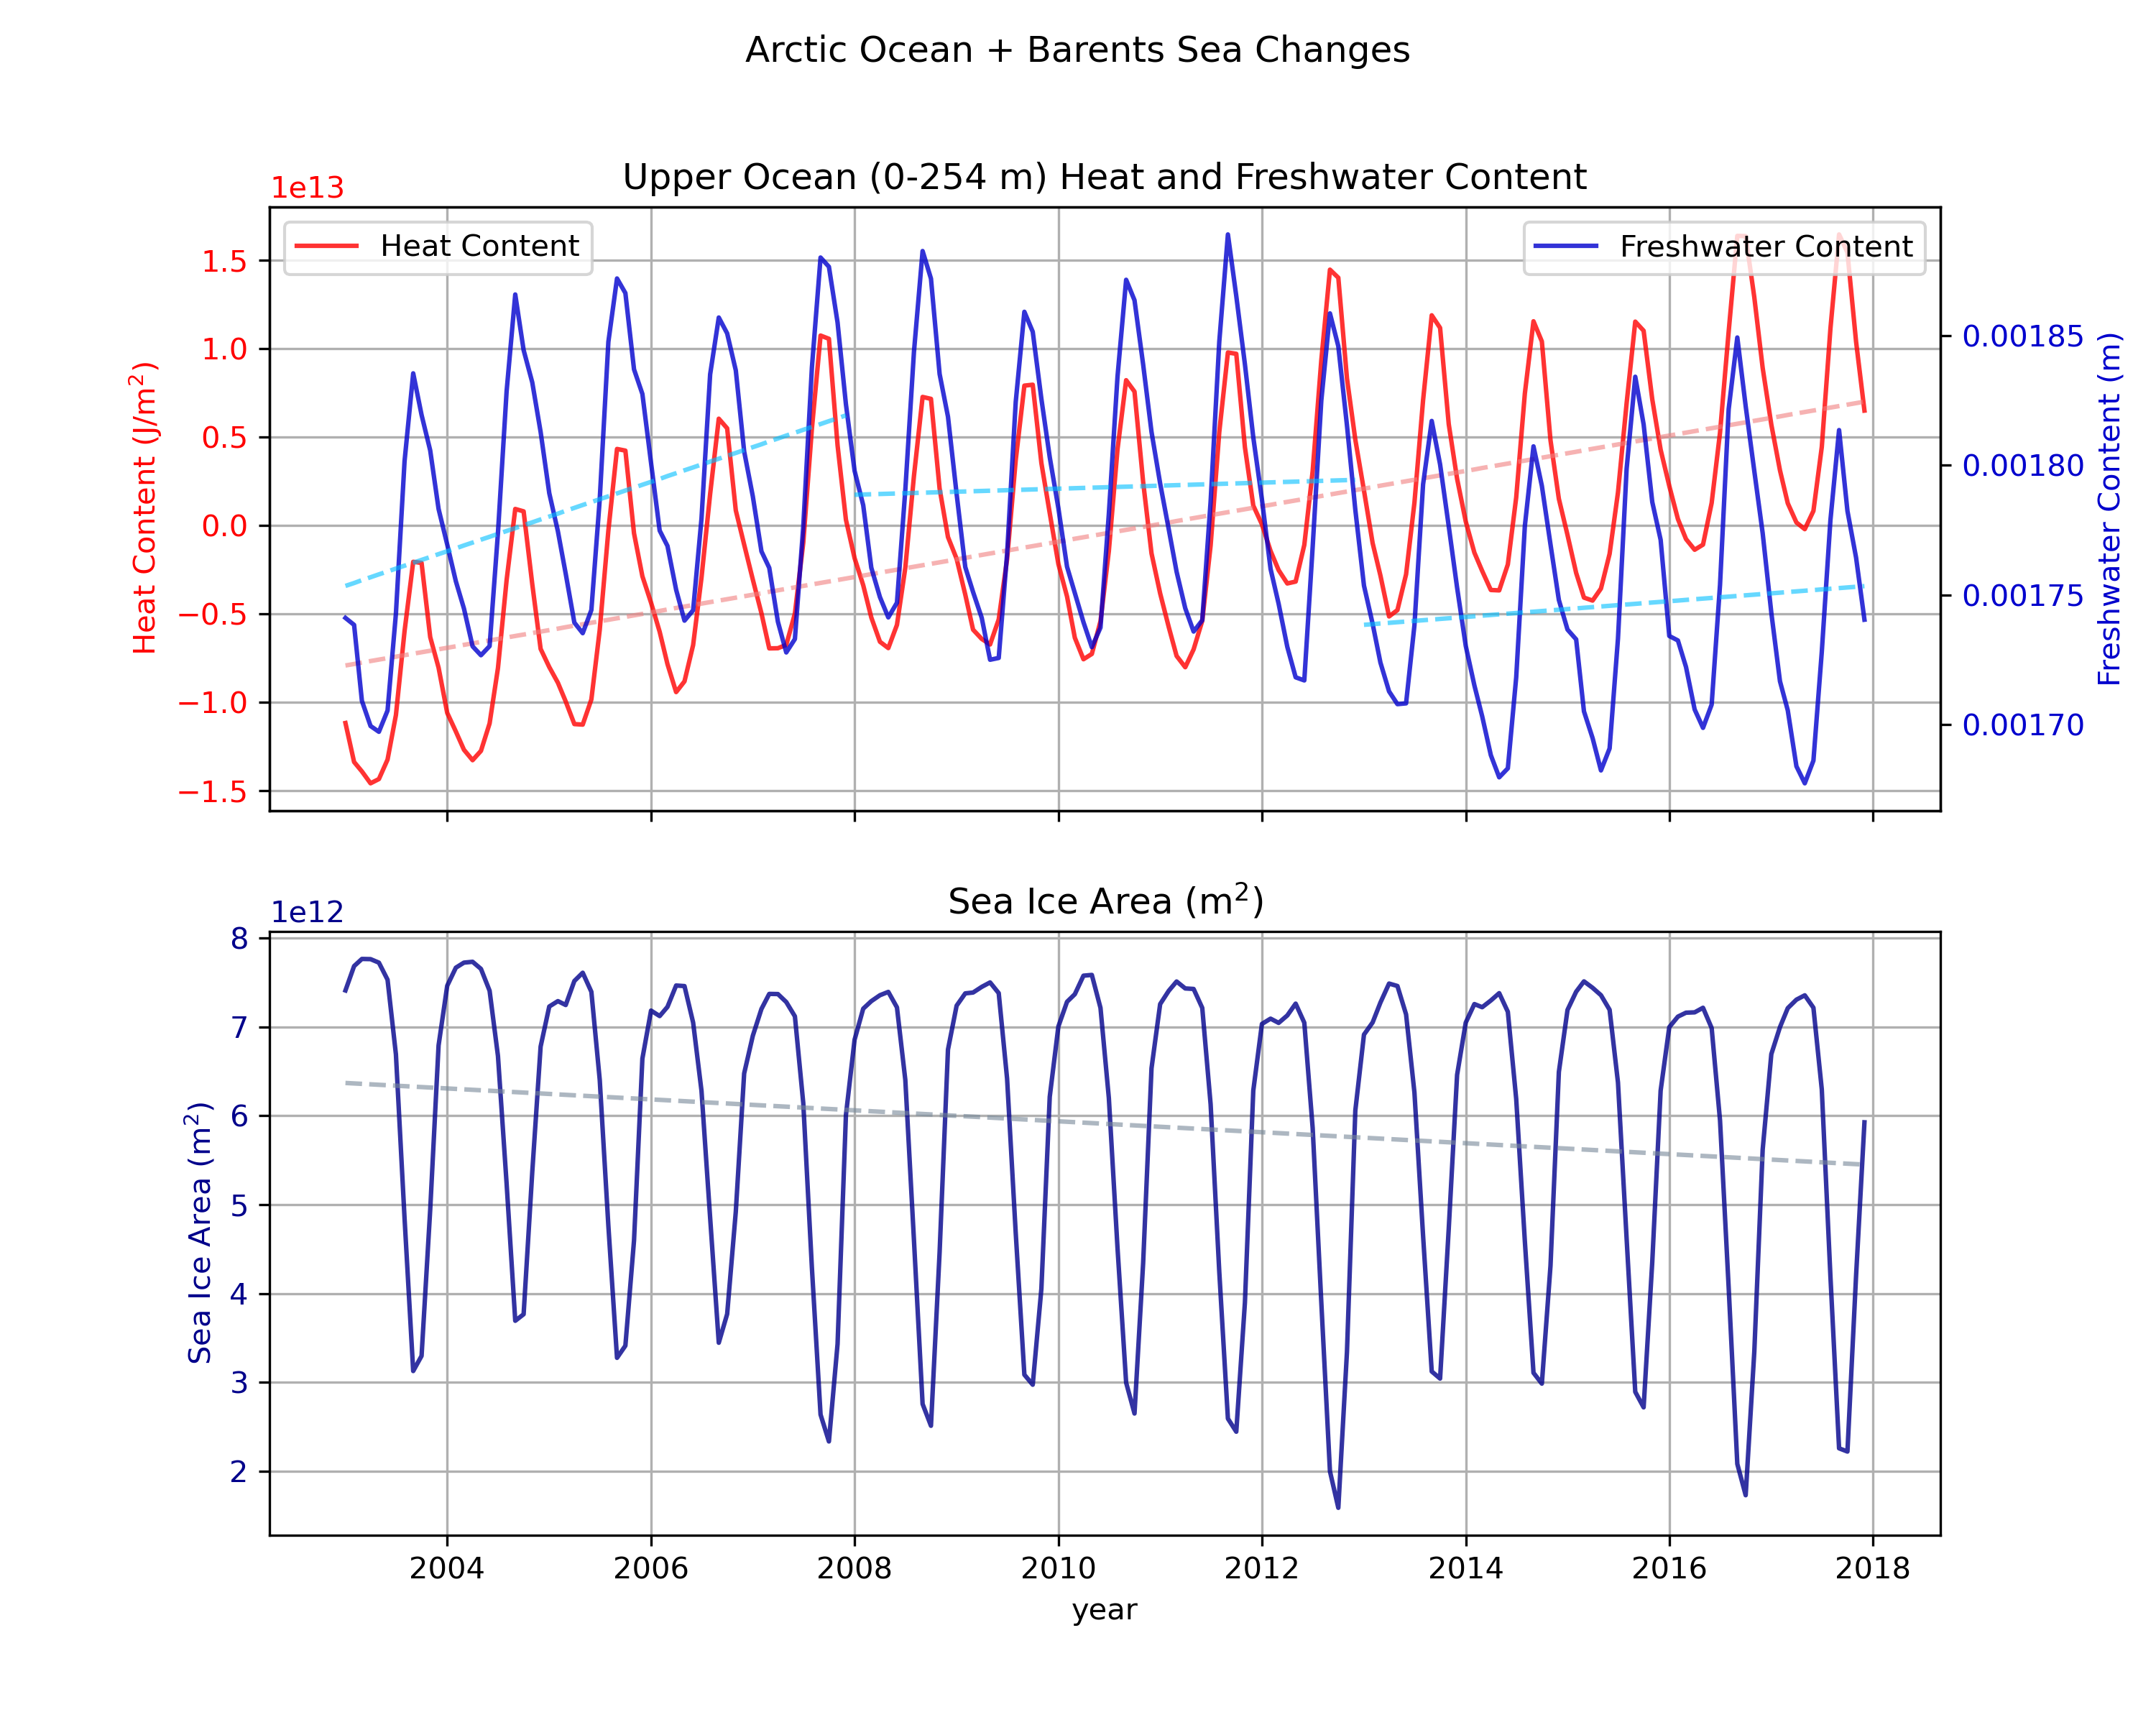
\includegraphics[width=\linewidth]{../figures/Arctic_timeseries_proposal.png}
        \caption{Top: Upper ocean heat and freshwater content across the Arctic during the ASTE time period. Heat content is steadily increasing, as shown by the dashed red line. Freshwater content increased from 2002--2007, declined from 2012--2014, then increased again from 2014--2017, as shown by the blue dashed trend lines. Bottom: Sea ice area in the Arctic, on a steady decline over time as shown by the gray dashed trend line.}
        \label{fig:arctictimeseries}
        \end{wrapfigure}


        % arctic atlantification
        One of the key changes to the Arctic in recent decades has been Arctic "Atlantification", the process whereby increasing amounts of AW is supplied to the Arctic Ocean through the Atlantic gateways. This water gradually expands to the central Arctic Ocean, changing the physical and biological characteristics of the Arctic to be more similar to the Atlantic \cite{Ingvaldsen2021}. In recent years, increased heat transport from the Atlantic gateways has accelerated these changes \cite{Arthun2012}. Studies have noted a key role for the Barents Sea Opening (BSO) as a part of this process. Here, OHT plays an important role in sea ice decline for the Barents Sea \cite{Li2017,Lind2018}, as well as for the internal Arctic \cite{Arthun2019}. Thus, understanding the implications of OHT through Atlantification, both in the past and at present, is vital to analyzing the heat changes of the Arctic Ocean.

        % introduction on several studies
        Several studies have analyzed the origin of increasing heat and freshwater content in the Arctic \cite{Haine2015,Polyakov2017}. Many of these studies have focused on local impacts of vertical mixing on heat and salt fluxes \cite{Polyakov2020,Lundesgaard2022,Schulz2022}, changes to gateway transports \cite{Oldenburg2024}, and the impact of reduced sea ice cover on the ocean heat transport \cite{Timmermans2018}. In other words, they analyze the impact of the changing climate on the heat or salt change. Despite the interest, few studies have analyzed the changing heat and salt of the Arctic simultaneously. By limiting these changes in ocean properties, analysis on the changes in ocean density, or water mass transformation (WMT) are missing in som studies. Furthermore, many Arctic analyses have highlighted the need to understand the long-term implications of fresh and heat anomalies in the Arctic.

        % goals/aims/what is aste
        We utilize regional state estimation, the Arctic Subpolar gyre sTate Estimate (ASTE), built from the previous solution in ECCO \cite{Forget2015}, to resolve the heat and salt content of the Arctic Ocean and surrounding seas. Using fifteen years (2002-2017) from a data-constrained state estimate \cite{Nguyen2021}, we aim to quantify how the noted warming of the Arctic Ocean can be attributed to the change in sea ice extent, area and concentration, and that these changes allow for advection of AW to the central Arctic. The changing role of the Barents Sea is an important component of the Arctic heat budget \cite{Arthun2016}, and can be quantified by budget analysis. We anticipate the respective role of the sea ice as a surface process on the buoyancy changes of the Barents Sea and the Arctic to explain the temperatures and salinity changes in this region. Furthermore, because budget analysis has not yet been used in coordination with WMT, it has not yet been possible to quantify the respective role of horizontal advection as compared with vertical diffusion and other mechanisms in the atmosphere and ocean as impacts on ocean buoyancy.

        % Overarching goal
        The overarching goal of this project is to resolve the relative contribution of different forcing terms in ASTE to the changing Arctic Ocean, and to better understand changes to the mixed layer. Budgeted diagnostics will be used to diagnose the most important terms transforming AW as it circulates the Arctic, as well as its impact on the internal Arctic Ocean buoyancy. By identifying the most important long-term tendencies for WMT in the Arctic, we can begin to piece together the potential long-term effects of continued warming on the Arctic. Budgeted diagnostics resolved using ASTE will be used to diagnose the advection of Atlantic Water into the Arctic and resolve its heat loss in the Arctic Ocean, as well as its impact on the changing stratification of the Arctic. By using these diagnostics to reliably resolve and pinpoint, the most important processes to the changing climatology of the Barents Sea and the Arctic, we will resolve gaps in the understanding of these regions, paving the way for future climate research.
    
    %\newpage
    \subsection{State of the art}
    % what is TS analysis and why does this help us look at buoyancy
    The circulation of the global oceans depends on their stratification, determined by density, a product of salinity \emph{S} and potential temperature \emph{T}. The distributions of \emph{S} and temperature \emph{T} depend on several factors, including atmospheric fluxes, large-scale circulation, and vertical processes. In particular, the sea ice formation and distribution can play and important role on \emph{S} changes at the ocean surface, causing both freshening and salting of the water column, during the seasonal cycle of ice formation. One approach to studying buoyancy changes in the global ocean has been to translate the geographic distribution of ocean volume to explicitly defined \emph{T} and \emph{S} as coordinates. In \emph{T}--\emph{S} analysis, any measured point in the ocean is classified based on its thermohaline properties. Across an arbitrary basin, the total volume of water with the same thermohaline properties is classified as a water mass. 
    
    % one paragraph summarizing past WMT to the Arctic (Walin, Hieronymus, etc)
    First used to study WMT or flow across isohaline \cite{Walin_1977} or isothermal \cite{Walin1982} surfaces, analysis of volume transport in \emph{T}-\emph{S} space has been applied in several subsequent studies in the North Atlantic \cite{Speer1993}, across gateways to the Arctic \cite{Rudels2008}, and across the pan-Arctic domain \cite{Pemberton2015} to study regional WMT. A framework to formulate volume, heat and salinity budgets has also been developed in which a change in water buoyancy is shown as a vector in \emph{T}-\emph{S} coordinates \cite{Speer1993,Hieronymus2014}. An example of this is shown in Figure~\ref{fig:groeskamp}, where fluid volumes can be "transformed" by heat fluxes in the \emph{T} direction and by salt fluxes in the \emph{S} direction. Performing analyses in \emph{T}-\emph{S} space–rather than geographic space–allows for the quantification of dominant salinity or temperature driven processes in transforming distinct water masses.

    \begin{wrapfigure}{l}{0.5\textwidth} % 'r' for right, '0.5\textwidth' for width
    \centering
    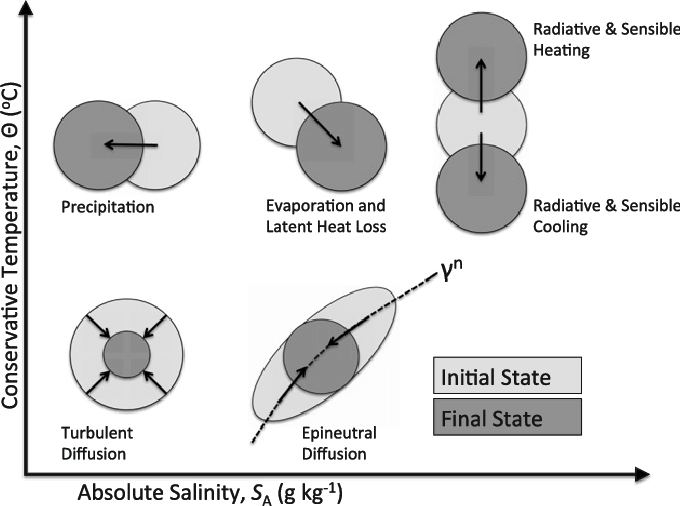
\includegraphics[width=\linewidth]{../figures/groeskamp_schematic.png}
    \caption{Several possible modifications to \emph{T} and \emph{S} in the ocean are possible. This schematic shows how fluid can be displaced through WMT. Arrows represent WMT, shaded regions depict volume distribution in \emph{T}--\emph{S} space, and $\gamma_n$ represents a surface of neutral density \cite{Groeskamp2014}.}
    \label{fig:groeskamp}
    \end{wrapfigure}

    % Barents Sea state of the art
    Ocean heat transport and heat loss to the atmosphere in the Nordic Seas have increased substantially over the last century due to the inflow of AW, making the Barents Sea a key warming hotspot for AW heat loss \cite{Smedsrud2022}. The Barents Sea is experiencing rapid changes to its heat and salt content \cite{Cosimo2014}, and recent studies of this region have noted changes both at the gate to the Atlantic Ocean and the gate to the Arctic. The BSO contributes most to ocean heat transport increases in recent years as compared with other gates to the Arctic \cite{Oldenburg2024}, and this heat transport from the Atlantic has been increasing in recent years \cite{Barton18,Wang2019}. At the opening to the Arctic, the winter import of sea ice has been in decline \cite{Lind2018,Lundesgaard2022}. Within the sea itself, recent studies have suggested that the Barents Sea is warming and freshening in recent years \cite{Skagseth2020}, with increases in downward heat transfer \cite{Lind2018}. Persistent sea ice loss over the last century has also meant a thinner CHL and weaker stratification \cite{Onarheim2017,Gerland2023}. There is evidence to suggest a positive feedback loop between the retreat of sea ice and subsequent decline in surface freshwater content, and the increase in heat content of the sea \cite{Arthun2012,Lind2018,Isaksen2022}. This is because with a weaker stratification, vertical mixing which heats the surface from AW below increases \cite{Lundesgaard2022}. Exposure of the ocean surface due to sea ice loss has played a small compensatory role to this heating below, but not greater than the heating impact \cite{Oldenburg2024}. Beyond the potential impact on the climate, studies highlight the borealization \cite{Lind2018,Isaksen2022} and eutrophication \cite{Downes2021} of this region with implications for local fisheries. Still, uncertainties remain surrounding the feedback mechanisms of how sea ice loss and temperature increases reinforce each other, as well as how the exact interactions between the AW inflow and changing sea ice extent. Furthermore, the long-term implications of the changing Barents Sea on the internal Arctic Ocean and the Atlantic Meridional Overturning Circulation (AMOC) remain unclear.

    \begin{wrapfigure}{r}{0.7\textwidth} % 'r' for right, '0.5\textwidth' for width
    \centering
    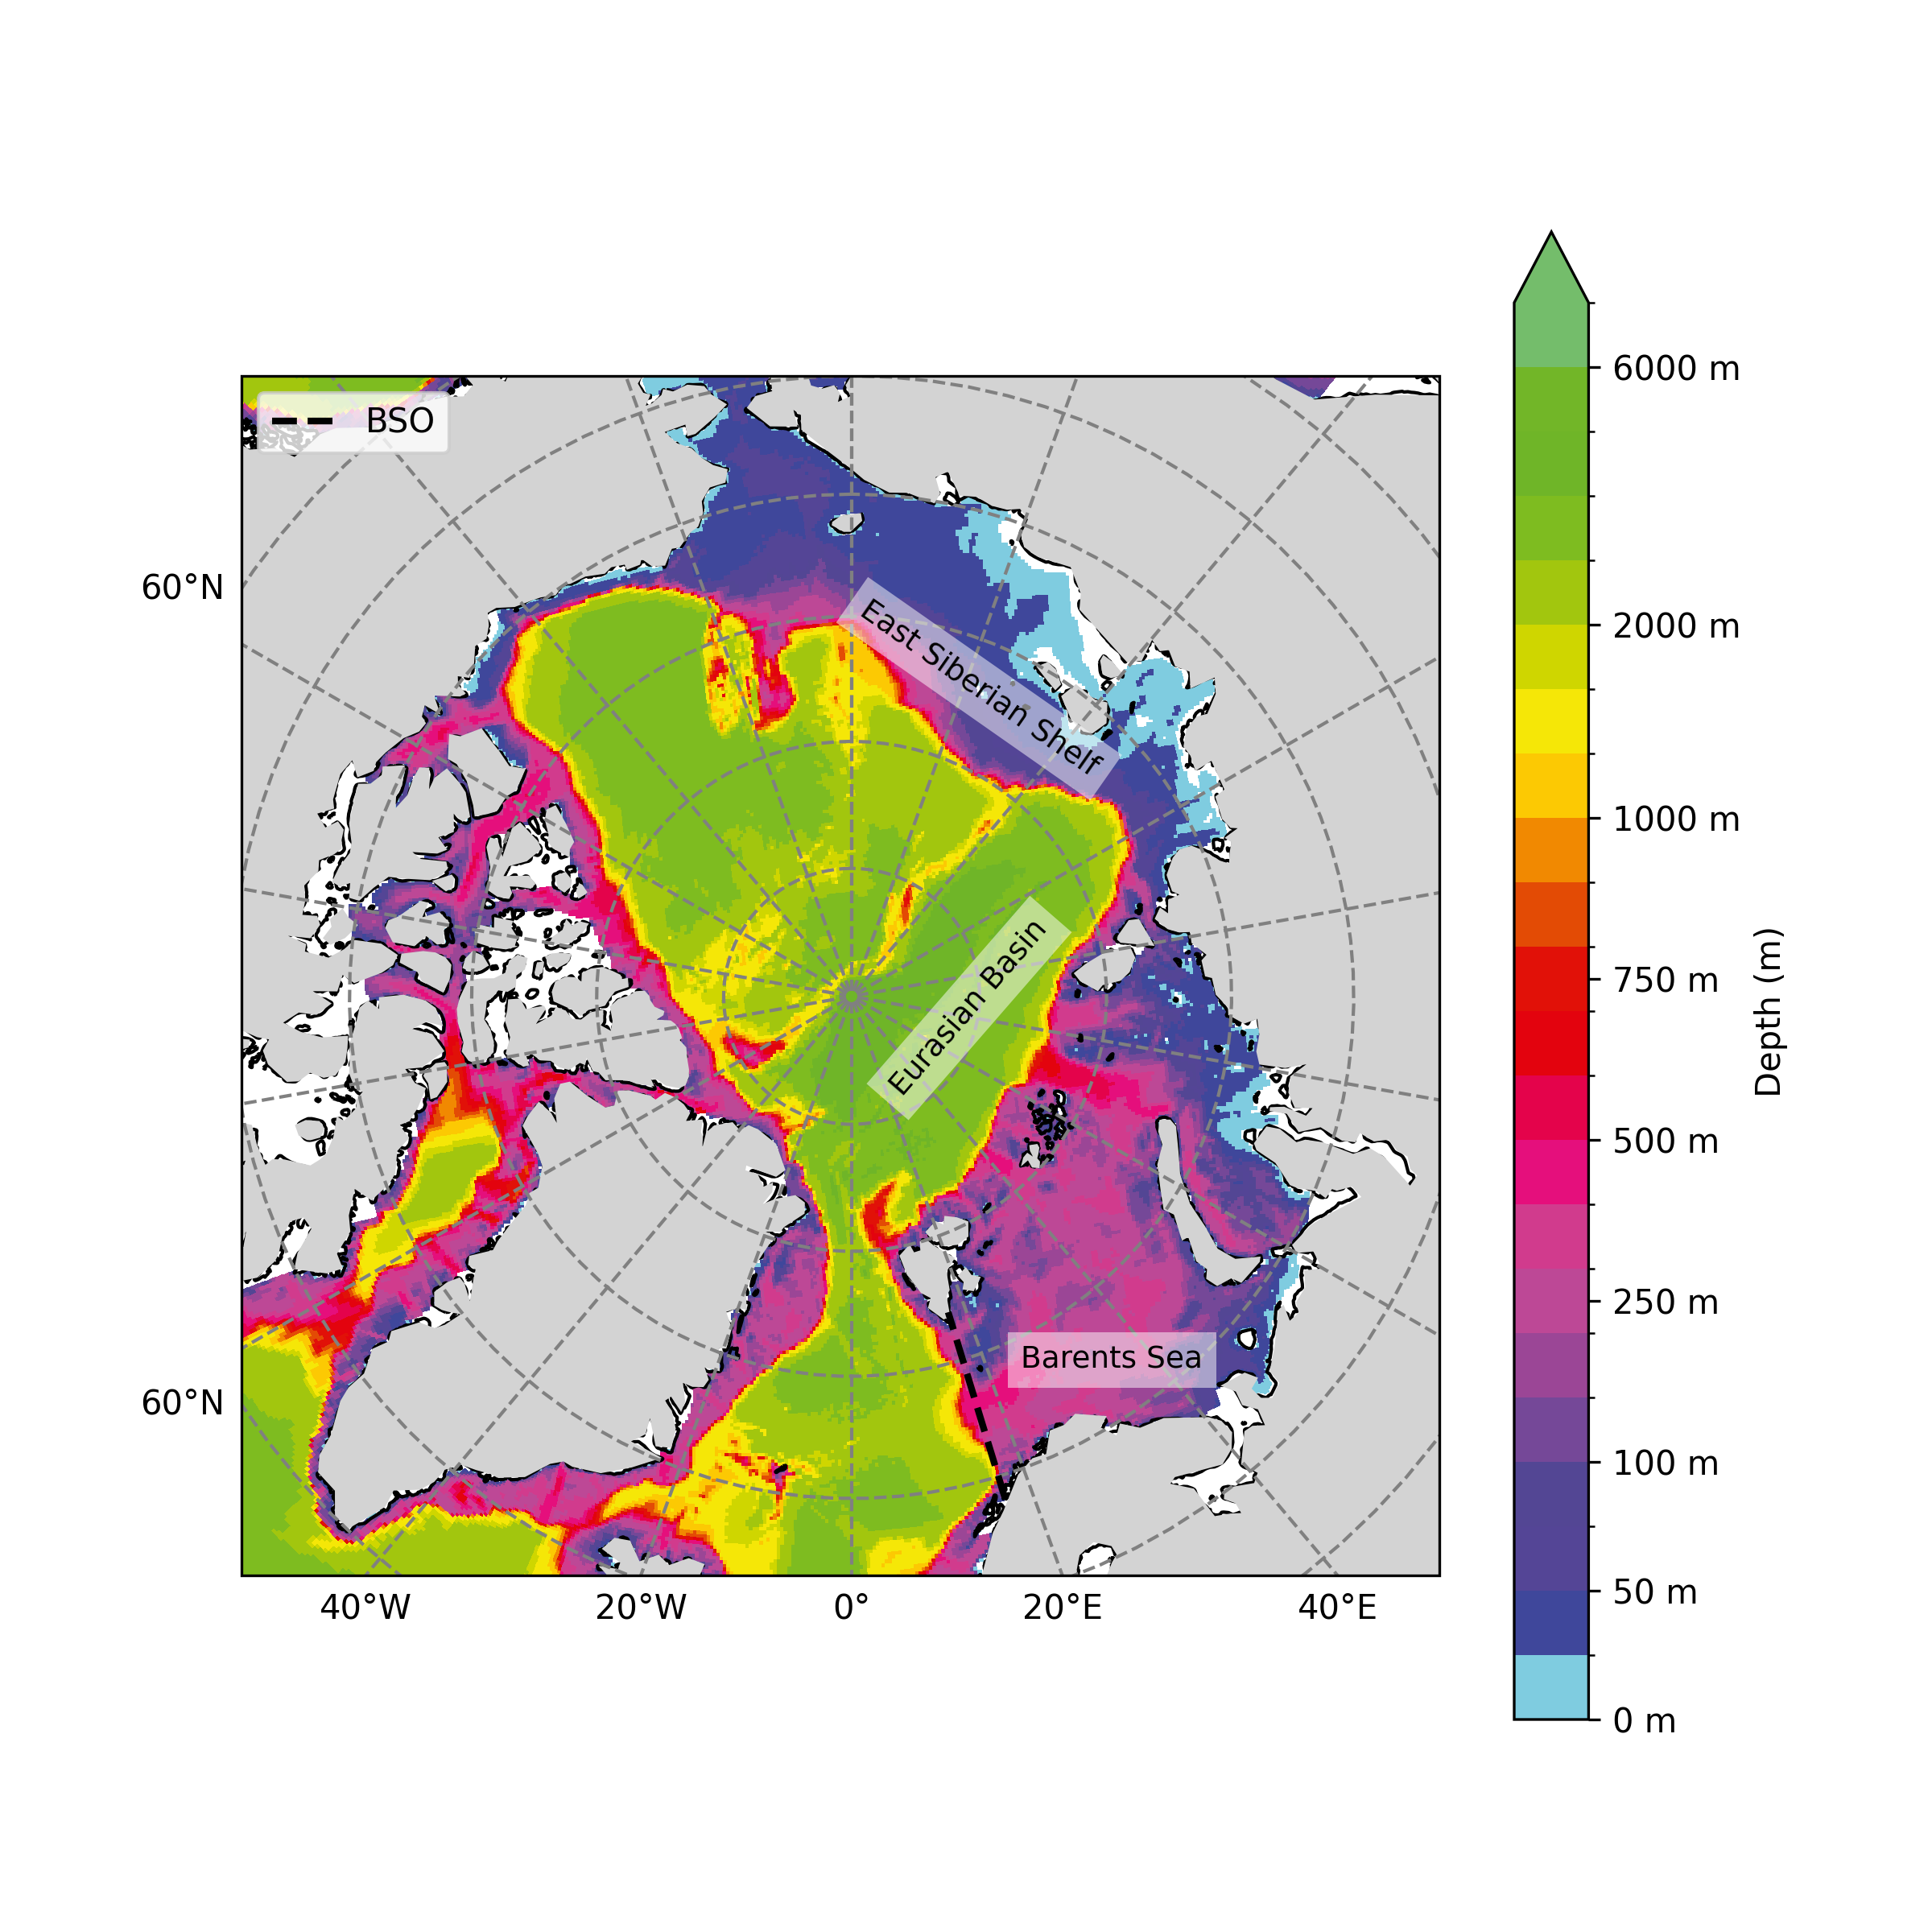
\includegraphics[width=\linewidth]{../figures/ASTE_bathymetry_labels.png}
    \caption{The bathymetry of the Arctic Ocean and marginal seas as represented in ASTE. Dashed gray lines show latitude and longitude and the depth of the seafloor is colored. A black dashed line shows the Barents Sea Opening, an important path for AW.}
    \label{fig:bathymetry}
    \end{wrapfigure}
    
    % Eastern Arctic studies
    Following the path of AW beyond the Barents Sea, the Eurasian Basin (EB) is also undergoing Atlantification and declining sea ice coverage \cite{Polyakov2017}. While AW was once only situated close to the surface near the Western Arctic, at the edge of the Barents Sea \cite{Schulz2022}, this shoaling has been observed farther East in recent years \cite{Polyakov2017} as well as increased shelf-basin exchange of water \cite{Williams2015}. The influence of AW has contributed to the weakening halocline both in the Eurasian Basin \cite{Polyakov2017} and farther east in the Makarov Basin \cite{Bertosio2022}, where the lower halocline is warming as a result of AW mixed with shelf water. Several important feedback mechanisms are associated with these changes to heat transport and sea ice retreat in the Eastern Arctic. In particular, reductions to albedo and subsequent increase surface heating in the summer \cite{Metzner2020} has increased summer heating of the mixed layer. Furthermore, as in the Barents Sea, decreased surface freshwater from sea ice melt has thinned the CHL, weakening stratification and increasing upward heat transfer to the mixed layer, where sea ice forms \cite{Polyakov2020}. One important driver of the upward heat transfer on the continental shelf is turbulent mixing, which can be driven by episodic wind-driven mixing \cite{Polyakov2020,Schulz2022} and is expected to increase with further sea ice reduction. However, observational studies of the Arctic are biased in the Eastern Arctic, making model analysis key in this region \cite{Lopez_Blanco2024}. Furthermore, the exact role of surface forcing, in particular how atmospheric forcing and sea ice changes effect vertical mixing, require further study. Analyzing the feedback mechanisms between ocean heat flux and sea ice processes is necessary to fully understand the heating of the East Arctic shelf. Thus, there exists a unique opportunity to study vertical mixing in coordination with sea ice forcing in this region.
    
    % discussion of this and other model studies; like Pemberton
    Developments in the \emph{T}--\emph{S} framework have been important to quantify the most dominant fluxes on ocean buoyancy in the Arctic, helping both to understand the past Arctic Ocean as well as predicting future stratification changes. However, budget analysis remains technically difficult, leaving uncomfortably large residuals in WMT studies, and making it difficult to analyze small-scale ocean processes beyond the most dominating terms \cite{Pemberton2015}. Thus, there still exist many uncertainties surrounding the role of specific processes in the Arctic responsible for the recent changes in heat and salt transport over the last decades. Closed budgets of heat, salt, and mass on the grid scale enable novel robust assessment of the relative roles of surface, advective and diffusive fluxes for the modification of water masses. Using budget analysis, we begin to unpack recent buoyancy changes in more detail, pinpointing exactly which processes are most responsible for the changing \emph{T}--\emph{S} distribution in various basins of the Arctic. These new diagnostics present a unique opportunity to exploit this method of analysis and fully understand the roles of each process on the changing Arctic Ocean.
    
    %\vspace*{5mm}

    %Objective and research questions
    %\newpage
    \section{Methodology}

    \subsection{Model description}\label{ASTE}
    % ASTE and what we can say about it
    We employ the Arctic Subpolar gyre sTate Estimate (ASTE), the coupled ocean-sea ice model that is an advanced version of the Massachusetts Institute of Technology general circulation model (MITgcm). The MITgcm solves the primitive equations using re-scaled $z^*$ coordinates with a fully non-linear free surface. The sea ice model is based on the framework described by previous models \cite{Menemenlis2005,Losch2010,Heimbach2010}. Tracer mixing and transports along isopycnals are also parameterized using previous literature.

    % what is the grid
    ASTE is based on the medium resolution LLC-270 grid, which at high latitudes is the equivalent of a cubed-sphere. The grid provides a nominal grid spacing of $1/3^\circ$, which corresponds to approximately 16 km in the Nordic Seas and 14 km in the Arctic interior. The ASTE domain covers the Atlantic northward of 32.5$^\circ$S as well as the entire Arctic and surrounding marginal seas and the Canadian Archipelago. The model is a "z-stepping" general circulation model with 50 vertical levels, thinner at the surface (~10 m) and thicker at depth (500-5000 m). Bathymetry is enforced with observations so as to realistically simulate transports along seafloor canyons and ridges. Because the bathymetry cannot be evenly discretized into these 50 levels, partial cells are are used to improve the topographic representation.

    % atmosphere forcing and TS valueThe atmospheric forcing in ASTE
    Lateral open boundary conditions are prescribed from the global ECCOv4r3 solution which is in agreement with in-situ and satellite constraints \cite{Nguyen2021}. Atmospheric forcing is applied using bulk formulae over the open ocean with initial conditions taken from JRA-55 reanalysis. Temperature and salinity stirring fields, or representation of mixing and redistribution processes of \emph{T} and \emph{S} by turbulence, eddies, and currents, are based on standard fields from the literature. These fields can be used to simulate how WMT occurs, particularly for small-scale eddies which are too small to resolve on the grid. 

    % ASTE and state estimation
    ASTE is constrained to $10^9$ satellite and in situ observations over the period 2002--2017. This approach works to minimize a cost function between the model outputs and observations so that the simulation outputs align as closely as possible with the real-world. To achieve this, the adjoint model is used which uses a process of algorithmic differentiation (AD), which computes a gradient-based least-squares minimization of the model data misfit, and at each time iteration, adjusts parameters to reduce the computed cost function. This process of optimization and strict adherence to conservation laws, ASTE enables analysis of closed budgets of heat, salt, mass, and momentum at the grid scale.

    \subsection{Budget analysis}

    % creating the budget generally
    Budget analysis is based on the conservation laws in the ocean. In the MITgcm these budgets is calculated from the ocean state, recorded at the beginning of each month in the time period from 2002--2017. For each grid cell in the LLC grid used in the model, we calculate three closed budgets: for heat, salt, and volume. For our results, we primarily focus on the budgets of heat and salt. Closing these budgets for the ocean is not a trivial matter, and there are several subtle differences one needs to be aware of. While salinity (units $g/kg$) and temperature (units $^\circ C$) fields are intensive quantities in the model, we create our budgets of heat and salt as extensive quantities. We express the terms contributing to the budget as a rate of change of these between two time snap-shots, such that an the salt budget for any cell (units $g/s$) or heat budget for any cell (units $J/s$), is the sum of all contributions to salt or heat from advection, diffusion, the nonlocal K-Profile Parameterization (KPP) scheme, and the surface forcing. Using this method, we can easily attribute any change in the salinity or heat to the terms used in the budget.

    \begin{wrapfigure}{l}{0.8\textwidth} % 'r' for right, '0.5\textwidth' for width
    \centering
    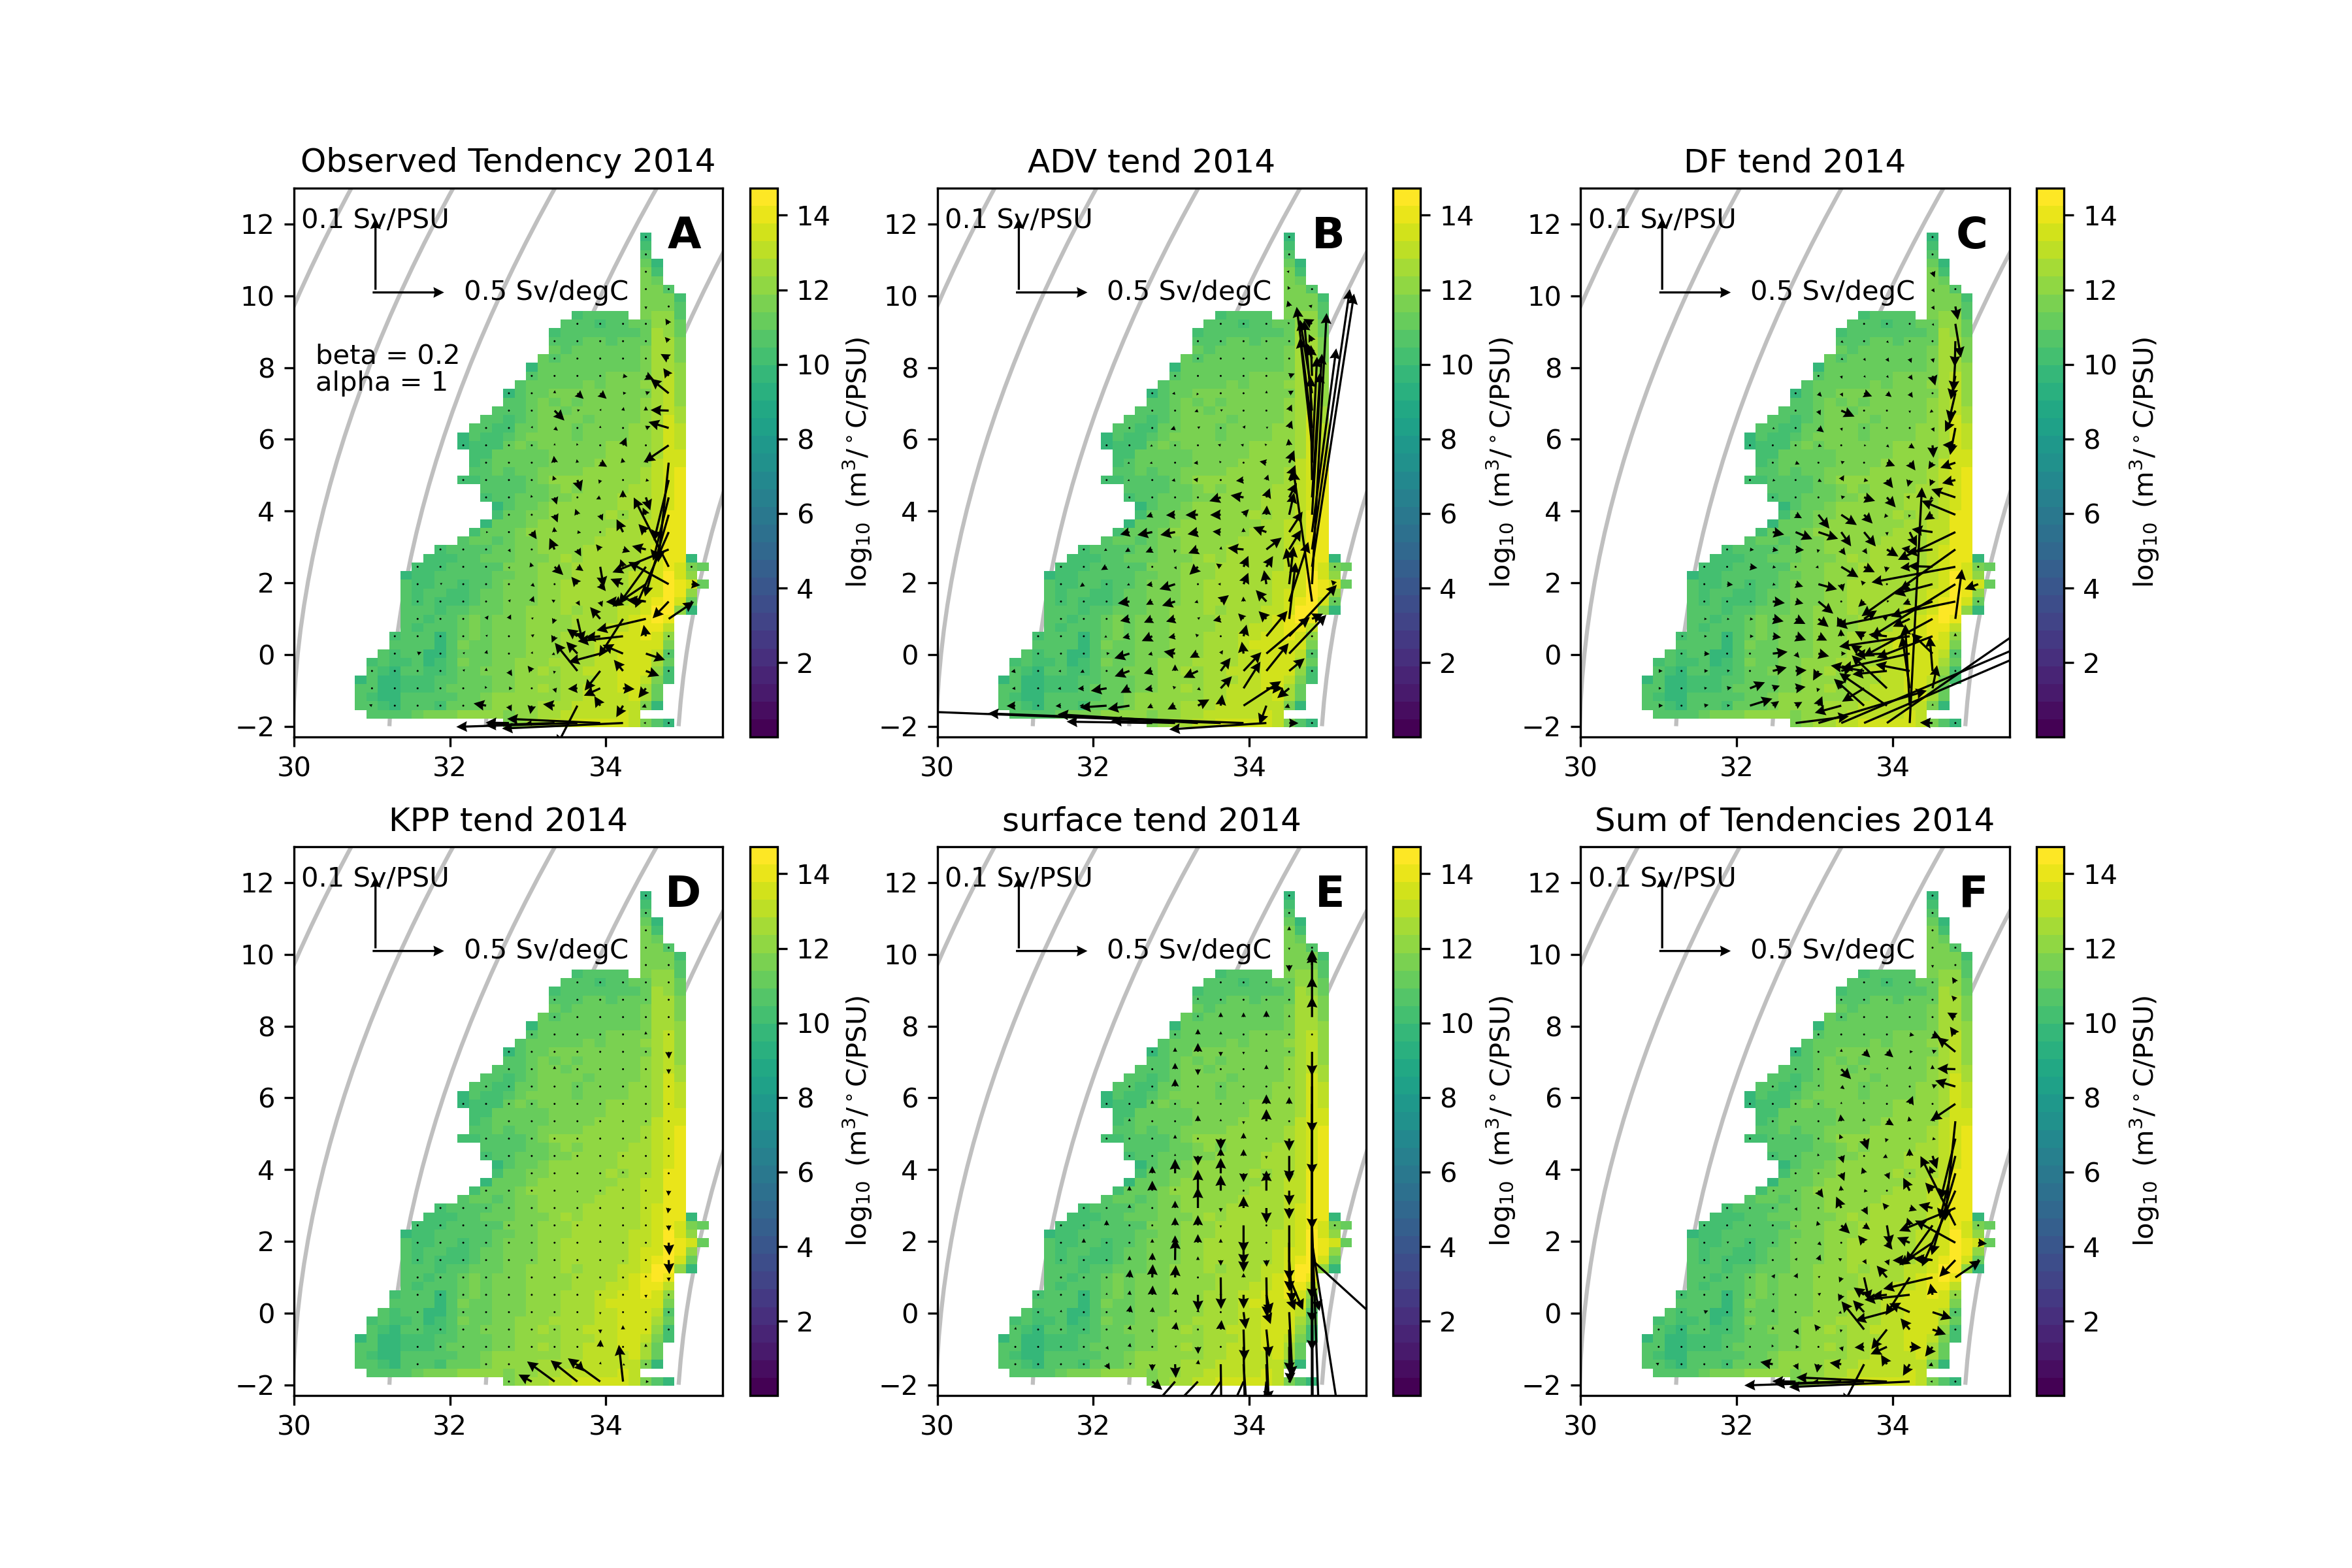
\includegraphics[width=\linewidth]{../figures/BarentsS_alltend_2014.png}
    \caption{\emph{T}-\emph{S} diagrams from ASTE Release 1 for the year 2014 in the Barents Sea, showing the net transformation calculated from the change in \emph{T} and \emph{S} over time (A), which is broken down into components due to advective (B), diffusive (C), KPP (D), and surface (E) fluxes. The sum of B-E is shown in F, which is equivalent to A.}
    \label{fig:sample_wmt}
    \end{wrapfigure}

    % INCLUDE ANOTHER PARAGRAPH ON THE BUDGET BREAKDOWN AND THE UNITS as similar to ECCO tutorial
    % https://ecco-v4-python-tutorial.readthedocs.io/ECCO_v4_Salt_and_salinity_budget.html

    % what important distinctions do we need; be clear we are not breaking down the ice budget here
    In this project, the surface forcing for heat includes shortwave radiation
    Surface forcing for salt combines freshwater from the atmosphere (evaporation, precipitation, and runoff) with freshwater flux from the ice freeze and thaw cycles. The total heat flux, similarly is a sum of other terms including the contribution to heat from the atmosphere and ice, including the latent heat of freezing. While total heat and salt flux are used in our initial budget analysis, these will be further broken down in preparation for project sub-component \ref{sec2_1}.

    
    % why is budget analysis important compared with previous analysis, why do we care about the residual
    In studying processes driving changes in heat and salt, ensuring there are no residuals is crucial because it confirms all changes in the system can be fully accounted for by the existing diagnostics. Because our budgets are closed, any presence of residuals would indicate some diagnostics was not accounted for in the attributions to heat and salt. This could distort the analysis and may lead to incorrect conclusions about the role of different mechanisms driving change. Our accurate budgeting is unique among studies of WMT because it ensures that all terms balance and that the results are a true reflection of the ocean dynamics.

    

    % include a figure of budgeted arrows to show sample results - maybe a map
    Preliminary results from this analysis are shown in Figure~\ref{fig:sample_wmt}. Here, plots show a color map of the volume distribution in \emph{T}-\emph{S} space as an average of the year 2014. The total tendencies in Fig.~\ref{fig:sample_wmt}A are calculated from the change in temperature $\frac{dT}{dt}$ and change in salt $\frac{dS}{dt}$, and normalized by the widths of bins in \emph{T} and \emph{S}. Fig.~\ref{fig:sample_wmt}B shows that advective fluxes primarily make the Barents Sea saltier and warmer. In this region, this impact is due to the AW inflow through the Barents Sea Opening. Fig.~\ref{fig:sample_wmt}C shows that diffusive fluxes have the impact of homogenizing Barents Sea Water. This is seen by the transformation of ending members of cold, fresh water and warm, salty water towards more central values of T and S. Fig.~\ref{fig:sample_wmt}E shows surface fluxes primarily lead to a transformation of Atlantic Water to cooler temperature. Fig.~\ref{fig:sample_wmt}D shows that KPP acts mostly at the freezing line to warm the water. Finally, Fig.~\ref{fig:sample_wmt}F is calculated as a sum of Fig.~\ref{fig:sample_wmt}B--E. Because ASTE is budgeted and there is no residual, we perfectly show that the breakdown of terms in Fig.~\ref{fig:sample_wmt}F is equivalent to Fig.~\ref{fig:sample_wmt}A.

    \subsection{Temperature-Salinity Analysis}
    
    % how is this translated to the T-S space
    To quantify contributions to buoyancy changes in a sample geographic region, we implement the WMT framework \cite{Walin1982,Groeskamp2014} to the budgeted output from ASTE. First, we create bins of \emph{T} and \emph{S} based on our domain. Next, we assign each grid cell in the ocean to these bins based on the monthly mean \emph{T} and \emph{S} values for that cell. Then, the volume of that cell is the integral of all cells in geographic space that fall within that range of \emph{T} and \emph{S} values. For ease of analysis in this coordinate system, we translate our salt budget for any grid square from units of $g/s$ to $\frac{PSU.m^3}{s}$ by dividing by the average density of the ocean. The heat budget is similarly translated from units of $\frac{J}{s}$ to $\frac{^\circ C.m^3}{s}$ by dividing by the density of the ocean and seawater specific heat capacity. Just as we integrated for volume, we integrate our forcing terms to get a transformation vector in each \emph{T} and \emph{S} bin, which is normalized by the bin widths in both dimensions. This represents the tendency of water in that range to warm/cool or freshen/salt due to specific processes. Because our model is budgeted, the sum of all forcing terms in \emph{T} and \emph{S} space is the total tendency of water in these bins.

    % why is this useful -- can read through first and think if necessary
    
    \section{Research Project}
    One primary research question guides our work: How do sea ice, atmospheric forcing, and the ocean influence the changing regimes of the Arctic Ocean? Understanding the precise impacts of various diagnostics is vital to understanding past warming and freshening of the Arctic Ocean. The ability to fully represent surface processes and advection as impacts on ocean buoyancy provides new insights on the impact of climate change on the Arctic. Furthermore, we hypothesize study of the Arctic Ocean in the Water Mass Transformation (WMT) will reveal similar regime shifts across different Arctic basins, despite regional differences. We address this issue with three primary work packages.

    % reread and decide if we should delete this
    Here I propose to perform a comprehensive study of the controls on Arctic WMT using budget analysis in ASTE with a focus on Atlantification and heat transport. This work will aim to address open questions within the field of Arctic Oceanography:

    \begin{enumerate}
        \item Q1: What are the relative roles of surface forcing, Atlantic inflow, and internal mixing in warming and salinfying the Barents Sea? What have been the most important long-term tendencies affecting the buoyancy in this region? \emph{(Project 1)}
        \item Q2: How does the interaction between sea ice forcing and vertical mixing over the East Arctic continental shelf contribute to observed regional heating? What is the exact role of surface atmospheric forcing and sea ice changes in driving vertical mixing in the East Arctic, and how do these processes influence the ocean heat flux and sea ice feedback mechanisms? \emph{(Project 2)}
        \item Q3: How can we relate atmospheric forcing and wind anomalies to the changing heat content of the Eastern Arctic, and more broadly the Arctic Ocean? What are the primary controls of the observed ocean heat transport changes on the shelf, and what are the implications of global climate change on this region?\emph{(Project 3)}
    \end{enumerate}

    % To answer these questions, we propose three hypotheses, which will guide the three projects we approach and serve as a basis to test our analyses:

    % \begin{enumerate}
    %     \item H1: Budget analysis will show that rapid warming and salinification of the Barents Sea are driven by changes to surface forcing, including by sea ice retreat. While advection plays a role in WMT, the enhanced role for surface processes has resulted in the net formation of warmer, saltier water masses.
    %     \item H2: In the Eastern Arctic, intensified Atlantic heat transport along the Eastern Siberian continental shelf, driven by vertical mixing, is the primary factor in reducing stratification and contributing to Atlantification. We hypothesize that the impact of sea ice retreat is in a positive feedback with increased internal mixing, and both allow greater heat transport in the mixed layer.
    %     \item H3: Adjoint reconstruction allows us to gain further insights into the changes to the mixed layer from results of Project 1 and 2. We hypothesize that by using a physics-based approach in the Eastern Arctic, density anomalies in the mixed layer can be attributed to wind stress and  atmospheric heat flux anomalies.
    % \end{enumerate}

    \subsection{Project 1: the Barents Sea in a changing climate: a key benefit of budget analysis}
    
    \begin{tcolorbox}[minipage,colback=Goldenrod,arc=10pt,outer arc=10pt]
    \centering
    \textbf{Method:}	\emph{Budget analysis for early and late years in ASTE}\label{sec1_1}
    \end{tcolorbox}

    % summary paragraph on structure of the Barents Sea
    Arctic warming is non-uniform and is amplified in the Barents and Kara Seas, which feature the strongest decline in winter sea ice concentration and some of the most rapid warming in the entire Arctic \cite{Screen2010,Cosimo2014}. The Barents Sea is often considered a doorstep to the Arctic Ocean, and its shallow mean depth of less than 1000 feet (Fig.~\ref{fig:bathymetry}) means that the effect of surface forcing is particularly pronounced here. Historically, the Barents Sea has acted as a buffer between the North Atlantic and the Arctic Ocean, cooling inflowing AW. However, recent climate shifts have diminished this cooling capacity \cite{Lind2018}. On the west, the Barents Sea is bounded by the BSO, connecting it to the Atlantic Ocean, and on the North between Svalbard and Novaya Zemlya it opens to the Arctic Ocean. There are two primary water masses--defined by discrete sets of T and S values--in the Barents Sea: cold, fresh Arctic Water in the CHL and salty, warm Atlantic Water (AW) in the Atlantic Water Layer. 
    
    % BROAD AIM: look at heat transport and causes of convergence in the barents sea
    The broad aim of this first project is to investigate the changing WMT budget of the Barents Sea to identify the most important long-term tendencies that cause convergence of water masses in \emph{T}--\emph{S} space. The rapid changes in the Barents Sea, in particular its salinity and temperature increases over time, have not been addressed using budget analysis. Furthermore, because this coastal sea is so shallow, small changes to the buoyancy can have substantial effects on the stratification, so it is important to resolve even small forcing terms. Here, we propose to analyze this region using budget analysis, so that all terms effecting the buoyancy are analyzed.

    % what data are we using - MAYBE MOVE THIS EARLIER DECIDE LATER
    Datasets used for this project are drawn from the ASTE release 1 \cite{Nguyen2021}. This contains snap-shots of the ocean variables at the beginning and end of each month, as well as time-averaged output. The budgets for heat and salt are calculated from these snap-shots, as well as the volume distribution. The temperature and salinity fields used to study WMT are taken from the time-averaged datasets. Other diagnostics which help us to understand the atmosphere and climate at a time step include sea ice extent and wind stress as well as precipitation, evaporation, and runoff are recorded as time-averaged values, but are not used in budget closure.


    % how are we using the budgets -- what time periods are we looking at
    Using the process described above, we obtain the transformation vectors due to advection, diffusion, KPP, and surface forcing. From this, we propose to focus our analysis on two, five-year periods: 2003--2007 and 2013--2017. The purpose of this comparison is to provide a broad overview of the two time periods and to demonstrate the changing terms in ASTE in early and late years of the model simulation. For these two periods, we aim to study the impacts of changing sea ice and surface forcing. This avoids the first year immediately after the spin-up, which may give spurious results. By comparing these two periods with a focus on the changes to the surface term, we focus on the formation of warmer, saltier water masses as a result of the surface term as compared with other forcing terms.

    % looking at convergence
    Other analysis will focus on the convergence in \emph{T} and \emph{S} space. 
    The focus of this paper will be on heat loss within the Barents Sea with a particular focus on the which terms cause a convergence of volume in warmer, saltier water masses in \emph{T}--\emph{S} space. Based on the convergence in \emph{T} and \emph{S} space, we will identify the long-term accumulation of buoyancy in a given class as well as the anomalies of these volumes.


    %Budget analysis will show that rapid warming and salinification of the Barents Sea are driven by changes to surface forcing, including by sea ice retreat. While advection plays a role in WMT, the enhanced role for surface processes has resulted in the net formation of warmer, saltier water masses.    
    \begin{tcolorbox}[minipage,colback=Goldenrod,arc=10pt,outer arc=10pt]
    \centering
    \textbf{Expected Results:}	\emph{A key role for surface forcing}\label{sec1_2}
    \end{tcolorbox}
    % what is the goal
    Upon completion of the analysis of this project, a closer examination of the long-term forcings in the Barents Sea will be completed. I will have both the forcing terms in \emph{T} and \emph{S} space as well as the convergence of volume due to these terms for the early and late years of the ASTE release 1. From a geographic view of the surface terms, preliminary results already show reductions to sea ice extent between the two time periods. Thus, in my analysis in \emph{T} and \emph{S} space, I expect to see less contribution of freezing to salinification of the water in later years of ASTE. I also expect to see a greater role for surface warming (represented by warmer \emph{T}, fresher \emph{S} bins) due to the decrease in sea ice extent.

    % what is the implication of the result
    If a trend appears for any one term between the two time periods, this would suggest it is responsible for the observed changes in this region. For example, if the magnitude of the advective term appears to shift between the two periods, the implication is that changes to AW inflow may responsible for the warming and salting of the Barents Sea. This can be confirmed by the plot of convergence, which will show what water masses are being formed or destroyed by advection. Comparing these sets of analyses will quantify any long-term tendencies in the Barents Sea, and determine governing forces on long-term heat and salt changes from the model output.

    % if this fails, what did we do
    If the convergence plots or transformation vectors show no clear relationship between the two periods, at minimum this project will have set up the WMT framework in ASTE with closed budgets. The tools used to create these vectors can be used on smaller timescales or to compare seasonal distributions, as well as used for future budget analysis.

    \subsection{Project 2: Exploring the dynamical underpinnings of the Eastern Arctic}

    %\item Q2: How is Atlantification changing the climatology of the eastern Arctic? How can we relate changing sea ice to the inflow of heat through the Eastern Arctic? How can we investigate the causes of Atlantification by examining the heat loss of AW?
    
    \begin{tcolorbox}[minipage,colback=columbiablue,arc=10pt,outer arc=10pt]
    \centering
    \textbf{Method:}	\emph{Applied budget analysis with a focus on surface forcing}\label{sec2_1}
    \end{tcolorbox}

    % structure of the Eastern Arctic and main currents
    The Eastern Arctic shelf is a dynamic region in the Arctic Ocean, influenced both by the inflow of warm, salty AW from the west and relatively fresh Pacific Water from the Bering Strait. AW inflow to this region stems from both the Fram Strait and the Barents Sea. As in the Barents Sea, the halocline of the Eastern Arctic largely prevents upward mixing of AW heat to the mixed layer and sea ice. The continental shelf is quite shallow with a mean depth of less than 1000 m, and historically, AW was not considered to have a substantial impact on the sea ice in this region. However, recent studies have shown AW may be playing an increasingly large role in sea ice retreat in the Eastern Arctic \cite{Carmack2015}.
    
    % BROAD AIM: changes to the mixed layer as a result of sea ice/winds
    % how do we build on the results of the previous paper
    We propose to address the causes of Atlantification in the Eastern Arctic in the second project of this proposal. Using the tools developed in Project 1 as a guide, we will turn our focus to the heat transport along the path of AW as it circulates the Arctic. The primary goal of this WP is to leverage \emph{T}--\emph{S} analysis to better understand the weakening of the CHL and causes of heat loss. While previous studies have suggested a positive feedback between the ice loss and upward heat transfer in this region , smaller-contributing processes have not been resoled through budgeted analysis. In this study, we aim to fill gaps in previous studies beyond the most dominant forcing terms typically provided in other ocean general circulation models. 

    % central question
    As in section \ref{sec1_1}, we aim to track the long-term tendencies influencing heat in the Eastern Arctic and evaluate how these terms are changing Arctic Ocean water mass distributions. Project 1 used the budget of the ocean at the surface without a full breakdown of the terms contributing to sea ice formation or melt. The budgets for sea ice can be further decomposed, and includes terms such as the contribution of sublimation, snow on top of the ice, and latent heat of freezing. Fully budgeting the ice to the atmosphere and ocean fluxes may require additional diagnostics from the ASTE Release 1 \cite{Nguyen2021}. This will be an opportunity for modification of the budgeting scripts and allow us to see which diagnostics contribute the most to surface forcing.

    % expected results
    After budgeting the sea ice, we will build upon long-term tendencies identified in Project 1, focusing on the evolving internal mixing and stratification changes over the ASTE period. Alongside our analyses in \emph{T}--\emph{S} space, we will study also the time-evolving stratification and diapycnal mixing in geographic coordinates along the path of AW. Here, we will look specifically for changes to the forcing from sea ice along the trajectory of AW. By tracking the stratification changes alongside the transformations due to sea ice and internal mixing, we aim to derive a relationship between these terms. Studying how these terms are correlated and how they evolve with time will help address our hypothesis.
    
    \begin{tcolorbox}[minipage,colback=columbiablue,arc=10pt,outer arc=10pt]
    \centering
    \textbf{Expected Results}	\emph{Relating the role of sea ice and atmosphere}\label{sec2_2}
    \end{tcolorbox}

    % anticipated results
    Successful results from this project will show the most important terms effecting sea ice growth and distribution on the Eastern Arctic shelf. We expect there is a positive correlation between declines in sea ice due to atmospheric forcing and declines in vertical stratification of the ocean. Once the relationship between sea ice and internal mixing is identified, intermodel comparison with other WMT studies is possible, which will help us identify the improvements of budget analysis from other models. Furthermore, this will build our understanding of this region prior to starting Project 3.

    % model development in ASTE

    \subsection{Project 3: Adjoint sensitivity in the Eastern Arctic}

    \begin{tcolorbox}[minipage,colback=mossgreen,arc=10pt,outer arc=10pt]
    \centering
    \textbf{Method} \emph{Studying controls on salt content of the mixed layer using the adjoint method}
    \end{tcolorbox}\label{sec3_1}

    %\item Q3: What controls anomalies in the stratification of the Eastern Arctic? What are the most substantial drivers of changes in buoyancy and on what timescales are these important?

    %\item H3: Adjoint reconstruction allows us to gain further insights into the changes to the mixed layer from results of Project 1 and 2. We hypothesize that by using a physics-based approach in the Eastern Arctic, we can identify the timescales on which salt dynamics in the mixed layer can be attributed to surface forcing.

    % BROAD AIM: adjoint sensitivity study focused on mixed layer salt
    The aim of the third and final project will be to find the causal relationship between atmospheric variability and recent changes to OHT in the Eastern Arctic. In Projects 1 and 2, we study the impacts of surface forcing changes from the years captured in the ASTE R1 on the buoyancy changes of the ocean. In other uses of traditional forward modeling of the ocean, the initial conditions are altered in several case studies to examine the impact on the final modeled state. However, because the range of possible initial perturbations for a model can be vast, it can be helpful to apply the adjoint method to quantify the sensitivity of some output to all possible inputs.
    
    % Adjoint sensitivity studies FIX AND EXPAND
    %\cite{Heimbach2011,Pillar2016,Smith2019,Nguyen2020}.
    The adjoint method is a powerful tool to quantify the sensitivity of a single output to a range of possible inputs. In our case, the adjoint model determines the gradient of an output with respect to all input variables and established a causal link between the output of interest and the factors that influence it. By implementing algorithmic differentiation, the adjoint model back-propagates sensitivity information, and allows us to assess the influence of each input in geographic space and time. This method can help explain variability in a variable of interest by showing how various mechanisms lead to that change \cite{Pillar2016,Nguyen2020}. 
    
    % how will we do this with the adjoint method
    To use the adjoint method for this project, we set an objective function, here the OHT on the Eastern Arctic continental shelf. This objective enables us to evaluate all sources of variability affecting heat transport. The adjoint model computes sensitivities of this function to all control variables. These sensitivities, or gradients, are updated regularly and provide insight into how each variable contributes to the density variability in the mixed layer. The goal of this work is not only to find the largest sensitivities in geographic space, but also the lag at which specific control variable effect the objective.

    % also how we plan to synthesize ideas with previous projects
    Using the results from the previous two projects as a guide, Project 3 aims to provide a comprehensive understanding of the changing heat transport of the Eastern Arctic. By combining budget analysis from Project 2 with the adjoint method, we identify key drivers of stratification variability. Adjoint-based sensitivity maps produced from this work will help us to quantify the influences of atmospheric forcing, including wind stress, freshwater flux, and heat flux. Comparing these novel results with the forward-model budget analysis helps to produce a comprehensive study on the influences on heat transport. In turn, this will reveal the long-term implications of climate change on AW transport through the Arctic.
    
    \begin{tcolorbox}[minipage,colback=mossgreen,arc=10pt,outer arc=10pt]
    \centering
    \textbf{Expected Results} \emph{Attribution of stratification changes to atmospheric variability}\label{sec3_2}
    \end{tcolorbox}

    % the results we anticipate
    We expect to identify the dominant drivers of OHT anomalies in the Eastern Arctic, which will help us address our hypothesis that the influence of these factors are distinguishable. These results will identify the short- and long-term influences on heat transport, a proxy for AW influx to the Arctic. A publication on this work will build our understanding of how heat and salt accumulate in the mixed layer and guide broader oceanographic work quantifying uncertainties in this region.

    % if fail then what
    If the results of this study are inconclusive as, we will at the very least gain insights into the limitations of the adjoint method applied for this objective function. If we cannot prove attribution of this term to specific processes, this could underline the need for more work on model configurations or initial conditions. At minimum, the failure to model the objective function could still provide information on the adjoint sensitivity pathways, and might identify key regions or time frames in which the model is most sensitive to perturbation changes. Furthermore, even if we cannot successfully model the full nonlinear system, our work could still provide information on short-term attributions to OHT.

    
    %Methods
    %\newpage
    %\section{Outcomes and Significance of the Proposed Work}
	
     
    
    % you can find the template for this gantt chart in /figures/gantt_template.pptx, convert it to pdf and then to png to upload it on the document

    %example of a temporarily horizontal page
    \section{Work plan}
    The Ph.D. program was started in Fall 2023. Anticipating the defense in Fall 2027 and taking  the degree timeline will resemble the following:

    \begin{enumerate}
        \item \textbf{Coursework, literature review, and preparing budgeting scripts:} Fall 2023 -- Spring 2024

        Deliverable: Python scripts to perform budget analysis in ASTE
        
        \item \textbf{Project 1:} Spring 2024 -- Fall 2024
        
        Deliverable: publication on the configuration of budget analysis tools to study changes to the Barents Sea, with a focus on heat content changes
        
        \item \textbf{Project 2:} Spring 2025 -- Summer 2026

        Deliverable: publication synthesizing the influence of internal mixing versus surface forcing on the changes to the Arctic Ocean heat transport 

        \item \textbf{Project 3:} Summer 2026 -- Summer 2027

        Deliverable: publication on adjoint sensitivity to synthesize the impacts of atmospheric variability on OHT

        \item \textbf{Ph.D. Thesis:} Fall 2027

        Deliverable: Thesis
    \end{enumerate}
 %    \newpage
 % 	\begin{landscape}
	% \thispagestyle{mylandscape}
	% \vspace*{-3cm}
 %    \section{Timetable} 
 %    \begin{figure}[!htb]\vspace*{-0.4cm}
 %    \centerline{
 %    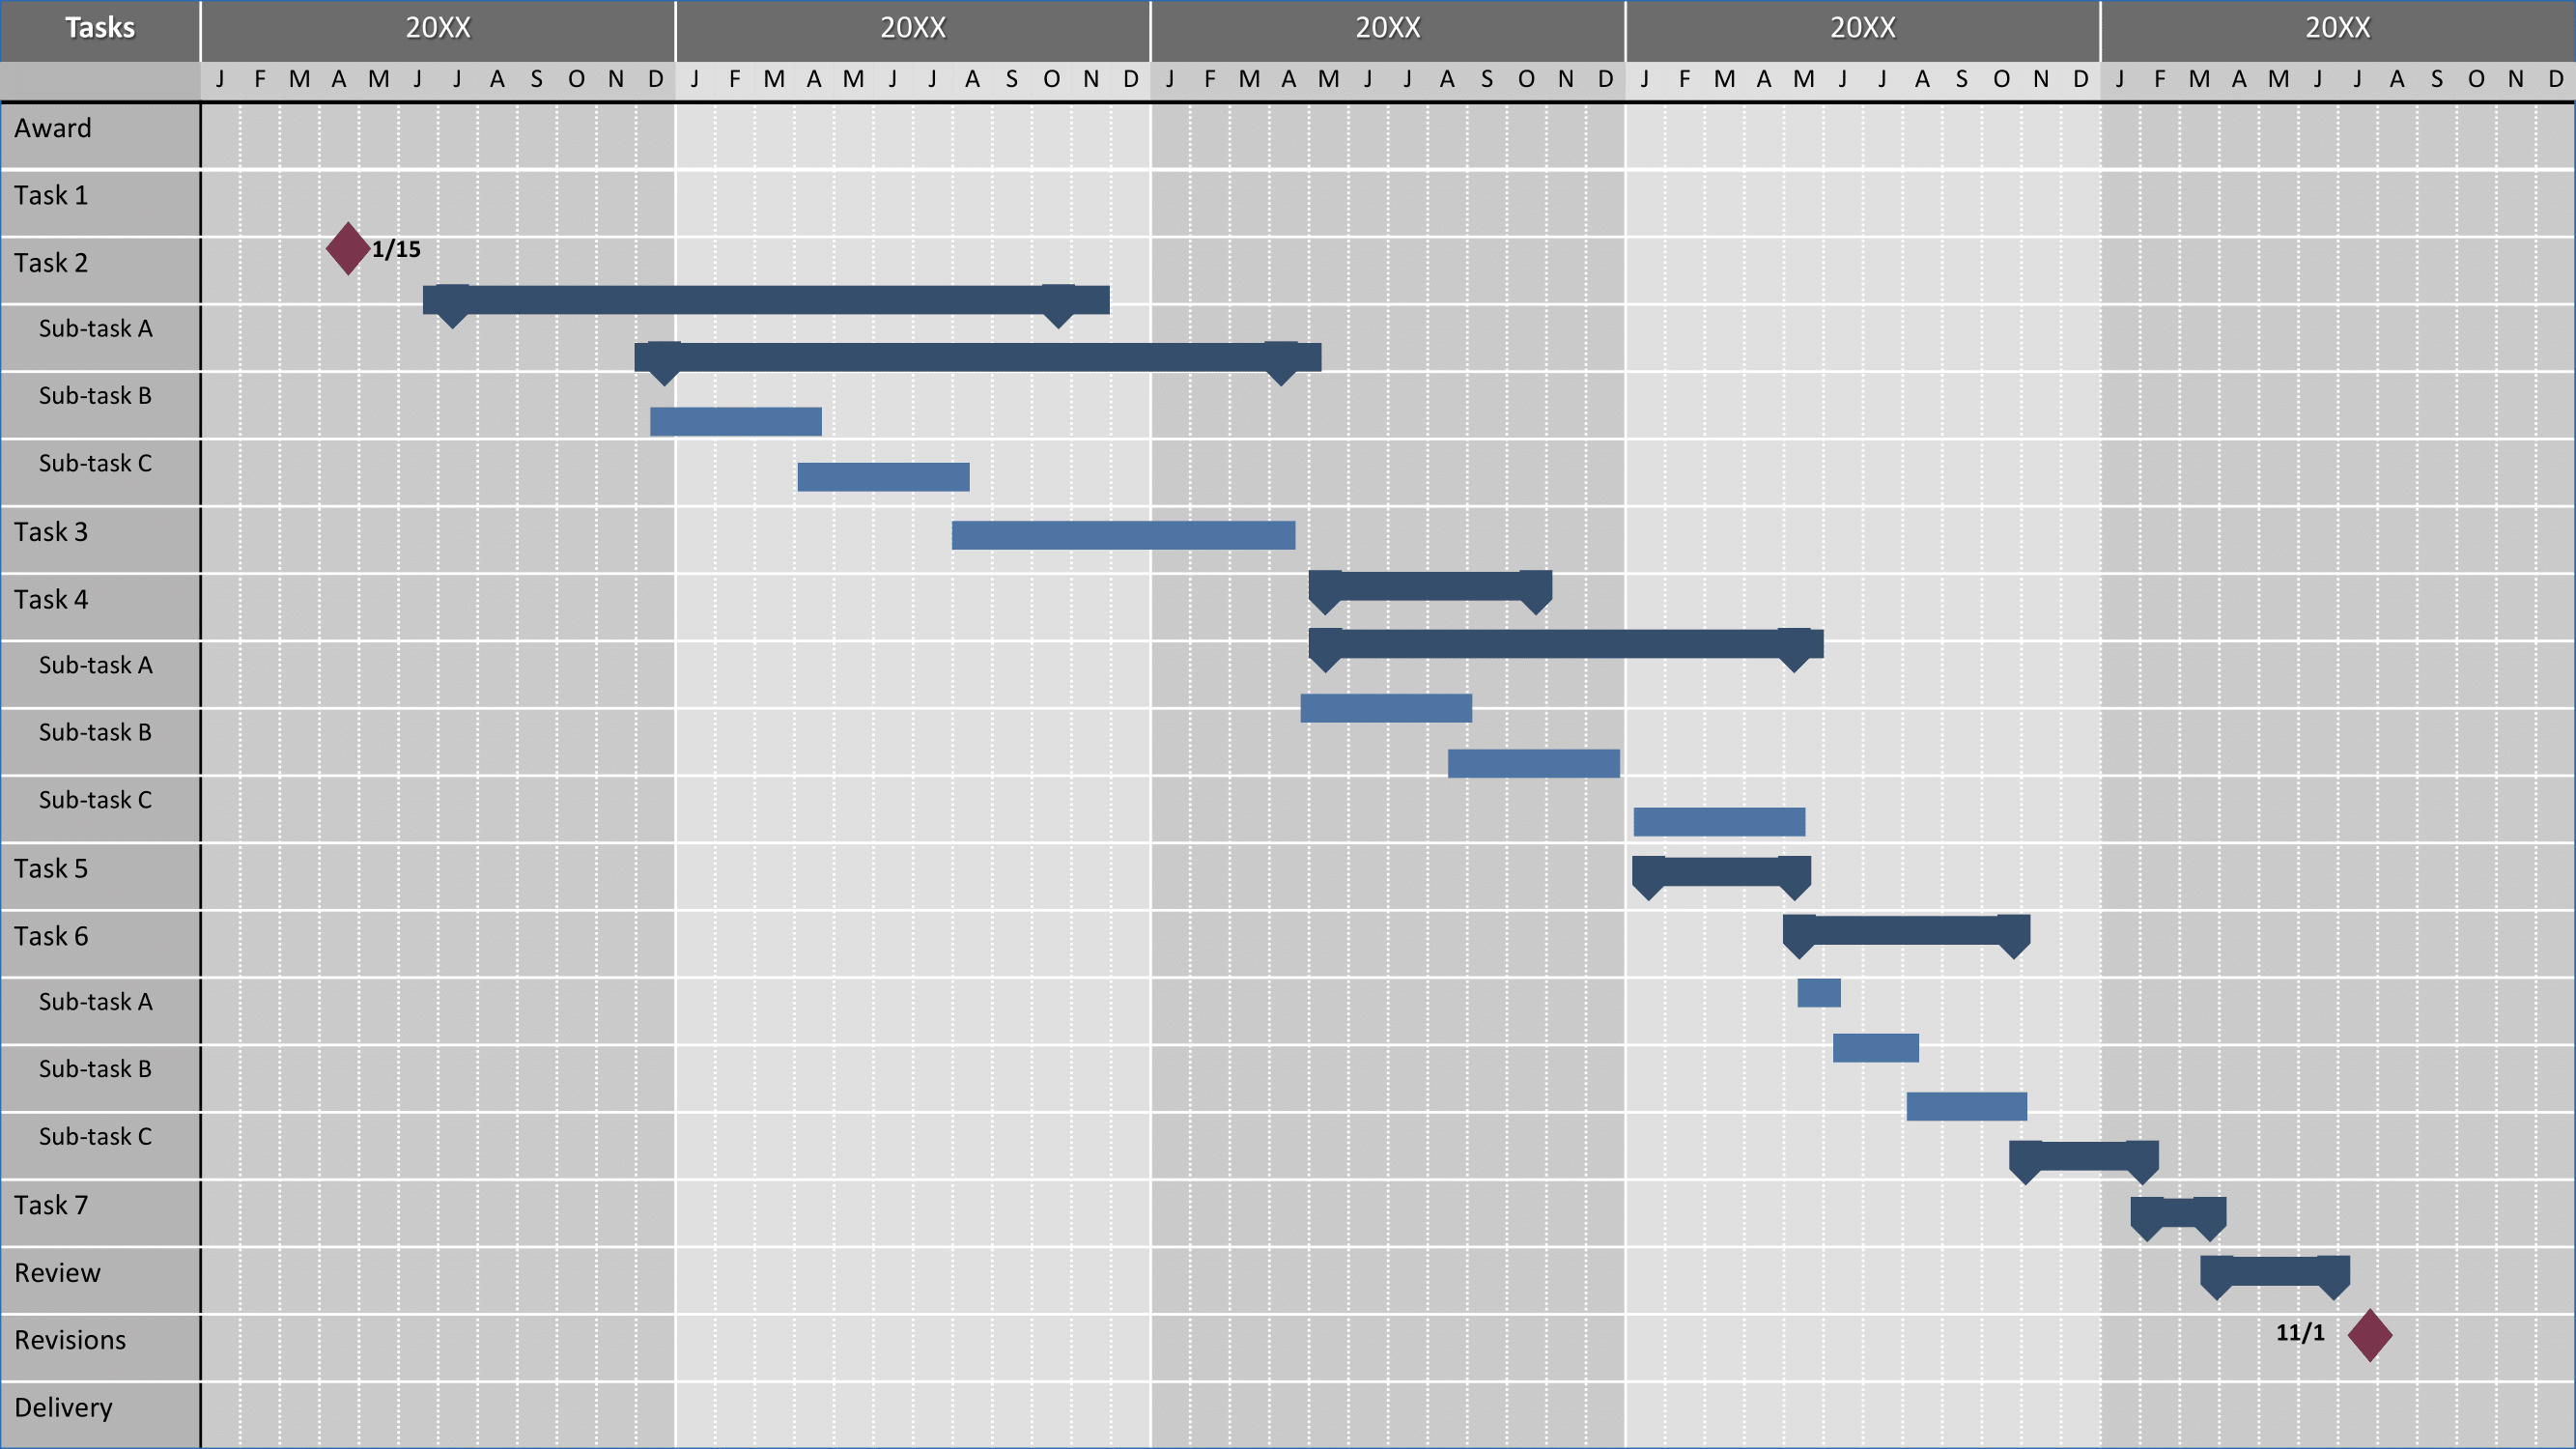
\includegraphics[scale=0.67]{../figures/gantt_template.png}
 %    }
 %    \caption{Gantt chart of the PhD project.}
 %    \label{fig:gantt}
 %    \end{figure}
 %    \end{landscape}
    

 		
% 	\newpage
% 	\section{Collaborations}
% 	\vspace*{1 cm}
%     \noindent \textbf{University - Department}\\
    
%     \noindent University address\\

% \textbf{Theme}

%     Person 1 - \href{mailto:<email>}{$<$email$>$} \\ \vspace*{-5.5mm}
    
%     Person 2 – \href{mailto:<email>}{$<$email$>$} \\

% \textbf{Theme 2}

%     Person 1 - \href{mailto:<email>}{$<$email$>$} \\ \vspace*{-5.5mm}

%     Person 2 – \href{mailto:<email>}{$<$email$>$} \\\\ 
   
    
% 	\section{Data management plan}
	
 	\newpage
% 	% references
	\addcontentsline{toc}{section}{References}

 \bibliographystyle{apacite}
\renewcommand{\arraystretch}{1.5}
\bibliography{references.bib} % Replace with your .bib file name
	%\bibliography{references.bib}

 %\printbibliography
	
\end{document}